\documentclass[11pt]{beamer}  %% versione proiettore
%%\documentclass[11pt,handout]{beamer} %% versione stampa
\usepackage{lucidiJb-2ed}

\usepackage{relsize}

\mode<article>
{
  \usepackage{fullpage}
  \usepackage{hyperref}
}

\mode<presentation>
{
  \setbeamertemplate{background canvas}[vertical shading][bottom=red!10,top=blue!10]
  \usetheme{Ethereum}
  \usefonttheme[onlysmall]{structurebold}
}

\subtitle{Learning Ethereum}
\title{Wallets}
\institute{Universit\`a di Verona, Italy}
\date{January 2020}

\setbeamercovered{invisible}

\def\codesize{\smaller}
\def\<#1>{\codeid{#1}}
\newcommand{\codeid}[1]{\ifmmode{\mbox{\codesize\ttfamily{#1}}}\else{\codesize\ttfamily #1}\fi}

\begin{document}

\begin{frame}
  \titlepage
\end{frame}

\begin{frame}
  \frametitle{Wallets}

  \begin{greenbox}{}
    A wallet is a software application that keeps track of keys.
    It creates and broadcasts transactions signed with those keys.
  \end{greenbox}

  \bigskip

  \begin{greenbox}{Public key cryptography}
    Private and public keys come in pairs.
    Ethereum uses private keys to create
    digital signatures for transaction authentication.
    Hence EOAs are controlled by a private key.
  \end{greenbox}

  \bigskip

  \begin{redbox}{}
    Data are not natively encrypted in Ethereum!
  \end{redbox}

\end{frame}

\begin{frame}\frametitle{Private/public keys from random numbers}

  \begin{greenbox}{Private key}
    In principle, just a random sequence of $256$ bits.
  \end{greenbox}

  \bigskip

  \begin{redbox}{Cryptographically-secure random generators}
    Private keys should be generated by using a cryptographically-secure
    random generator, or otherwise keys might not really be randomly
    spread and might be more easily guessed.
  \end{redbox}

  \bigskip

  \begin{greenbox}{Public key}
    It is computed from the private key, through a one-way function
    called \emph{elliptic curve multiplication} (ECDSA).
  \end{greenbox}

  \begin{center}
    The generation of a private/public key pair does not require any
    centralized service. The probability of computing an already used key
    is negligeable.
  \end{center}

\end{frame}

\begin{frame}\frametitle{Ethereum representation of the keys}

  \begin{itemize}
    \item A private key are 256 random bits: 64 hexadecimal digits
    \item A public key is a couple of two 256 bit numbers: Ethereum
      uses \<0x04> followed by $64\times 2$ hexadecimal digits
  \end{itemize}

  \bigskip

  There are libraries for computing public keys from private keys:

  \begin{itemize}
  \item OpenSSL (\url{https://www.openssl.org})
  \item libsecp256k1 (\url{https://github.com/bitcoin-core/secp256k1})
  \end{itemize}

\end{frame}

\begin{frame}\frametitle{Cryptographic hash functions}

  \begin{greenbox}{Hash functions}
    Any function that can be used to map data of arbitrary size to data of
    fixed size.
  \end{greenbox}

  \bigskip

  \begin{greenbox}{Cryptographic hash function}
    A hash function with the following properties:
    \begin{enumerate}
    \item determinism
    \item verifiability (in linear time)
    \item noncorrelation (small change of input induces extensive change of hash)
    \item irreversibility (\emph{one-way})
    \item collision protection: difficult to compute two inputs that produce the same hash
    \end{enumerate}
  \end{greenbox}
  
\end{frame}

\begin{frame}\frametitle{Ethereum's cryptographic hash function}

  \begin{greenbox}{Keccak-256}
    Ethereum uses the Keccak-256 cryptographic hash function.
    It is the original algorithm that won the SHA-3 Cryptographic Hash
    Function Competition of 2007. NIST standardized it in a slightly
    modified way as SHA-3. However, the Ethereum team never trusted
    such modification and used the original agorithm.
  \end{greenbox}

  \bigskip

  \begin{redbox}{Keccak-256 or SHA-3?}
    You can still see blogs and even the source code of Ethereum refer
    to SHA-3. Despite of that, \underline{Etherem does not use SHA-3}, but the original
    Keccak-256 algorithm!
  \end{redbox}

\end{frame}

\begin{frame}\frametitle{Derivation of an Ethereum address from the private key}

  \begin{greenbox}{}
    Compute the public key (without leading \<0x04>),
    hash it with Keccak-256, keep only the last 20 bytes (160 bits).
  \end{greenbox}
  
  \begin{center}
    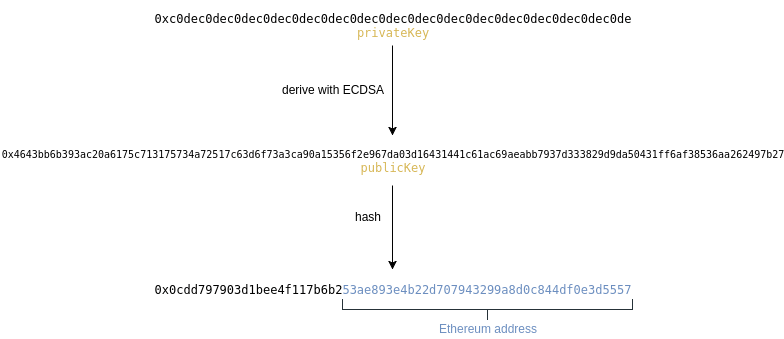
\includegraphics[width=\textwidth,clip=false]{pictures/ethereum-address-derivation.png}
  \end{center}

  \begin{center}
    No checksum!
  \end{center}

\end{frame}

\begin{frame}\frametitle{Checksummed address format: ICAP}

  \begin{greenbox}{}
    \<XE> + 2 characters of checksum + base-36 integer of up to 30 digits
  \end{greenbox}

  \bigskip

  \begin{greenbox}{}
    \begin{itemize}
    \item the base-36 integer can represent up to 155 bits, hence ICAP
      can only be used for addresses starting with a zero byte
    \item ICAP is compatible with IBAN
    \end{itemize}
  \end{greenbox}

  \bigskip

  \begin{greenbox}{Example}
    Ethereum address: \<0x001d3f1ef827552ae1114027bd3ecf1f086ba0f9>
    
    ICAP: \<XE60 HAMI CDXS V5QX VJA7 TJW4 7Q9C HWKJ D>
  \end{greenbox}

\end{frame}

\begin{frame}[fragile]\frametitle{Hex encoding with checksum in capitalization (EIP-55)}

  \begin{greenbox}{A backward compatible checksum injection}
    \begin{enumerate}
    \item use Keccak-256 to compute 64 hex digits from the uncapitalized Ethereum address
      (40 hex digits)
    \item capitalize each alphabetic address character if the corresponding hex digit
      of the hash is greater than or equal to \<0x8>
    \end{enumerate}
  \end{greenbox}

  \bigskip

  \begin{greenbox}{Example}
\begin{semiverbatim}
Address:   001d3f1ef827552ae1114027bd3ecf1f086ba0f9
Keccak256: 23a69c1653e4ebbb619b0b2cb8a9bad49892a8b9...
Result:    001d3{\color{red}F}1ef827552{\color{red}A}e111402{\color{red}B}7{\color{red}D}3{\color{red}ECF}1f086b{\color{red}A}0{\color{red}F}9
\end{semiverbatim}
  \end{greenbox}

  \bigskip

  \begin{greenbox}{Checking procedure of an EIP-55 encoded address}
    \begin{itemize}
    \item apply the above capitalization procedure to it
    \item the result must match the EIP-55 encoded address
    \end{itemize}
  \end{greenbox}

\end{frame}

\begin{frame}\frametitle{Nondeterministic wallets}

  \begin{greenbox}{Just a Bunch of Keys -- JBOK}
    They store one or more unrelated private keys, encrypted with a password,
    inside a keystore, ie, a textual file.
  \end{greenbox}

  \medskip

  \begin{greenbox}{Password stretching}
    To make dictionary attacks harder, they apply a hash function
    repeatedly to the password, using the hash result as actual encryption
    password. This is a so-called \alert{key derivation algorithm}.
  \begin{center}
    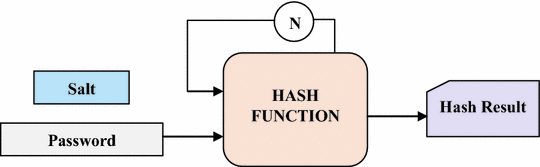
\includegraphics[width=\textwidth,clip=false]{pictures/key-derivation-function.png}
  \end{center}
  \end{greenbox}

\end{frame}

\begin{frame}\frametitle{Deterministic (seeded) wallets}

  \begin{greenbox}{Streams of keys}
    They store just a seed, from which streams of keys can be derived.
    \begin{itemize}
    \item the seed is the only information that must be stored and kept private
    \item each stream can be allocated for different goals or to
      distinct company departments
    \end{itemize}
  \end{greenbox}

  \medskip

  \begin{center}
    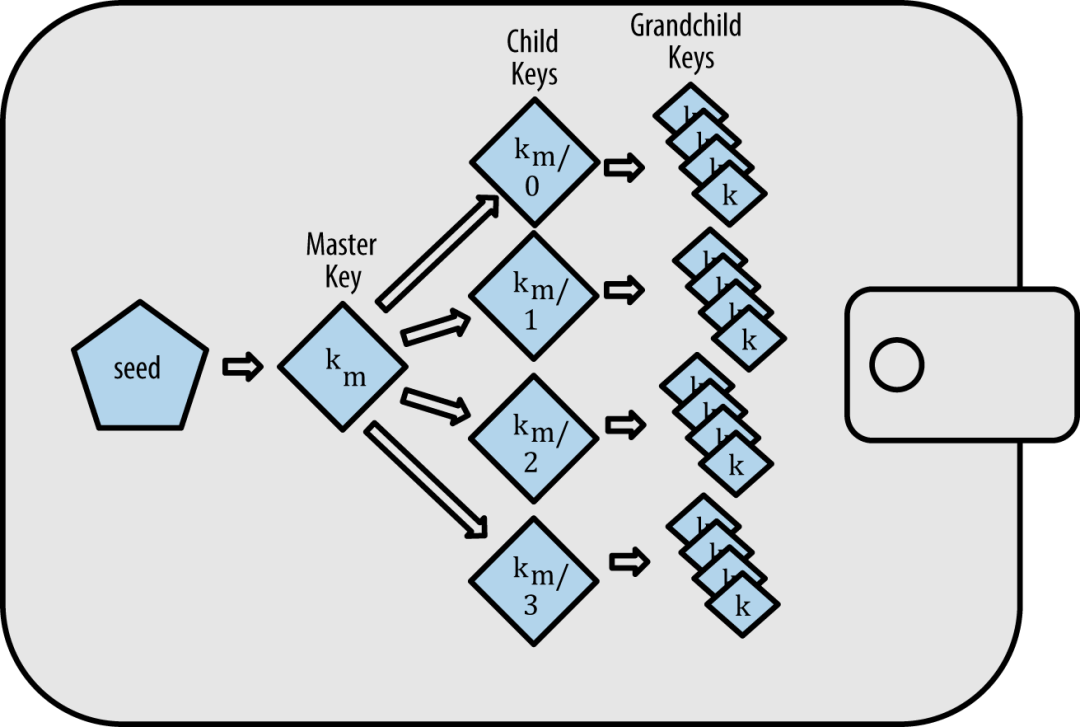
\includegraphics[scale=0.85,clip=false]{pictures/hd-wallet.png}
  \end{center}

\end{frame}

\begin{frame}\frametitle{Encoding the seed as mnemonic code words (BIP-39)}

  \begin{center}
    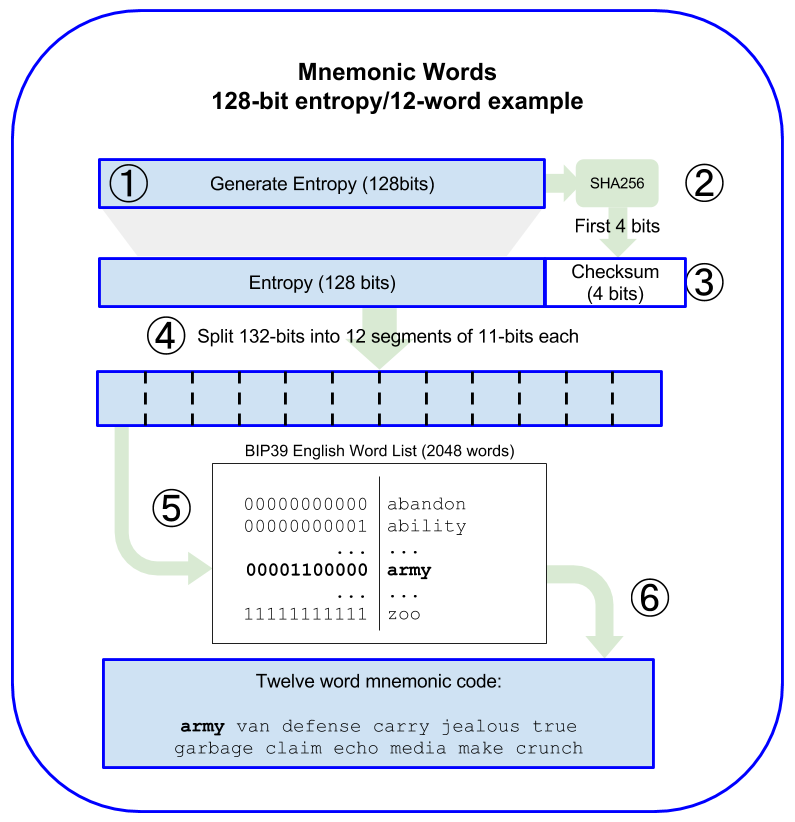
\includegraphics[scale=0.27,clip=false]{pictures/entropy-to-mnemonic.png}
  \end{center}

\end{frame}

\begin{frame}\frametitle{Encoding the seed as mnemonic code words (BIP-39)}

  \begin{center}
    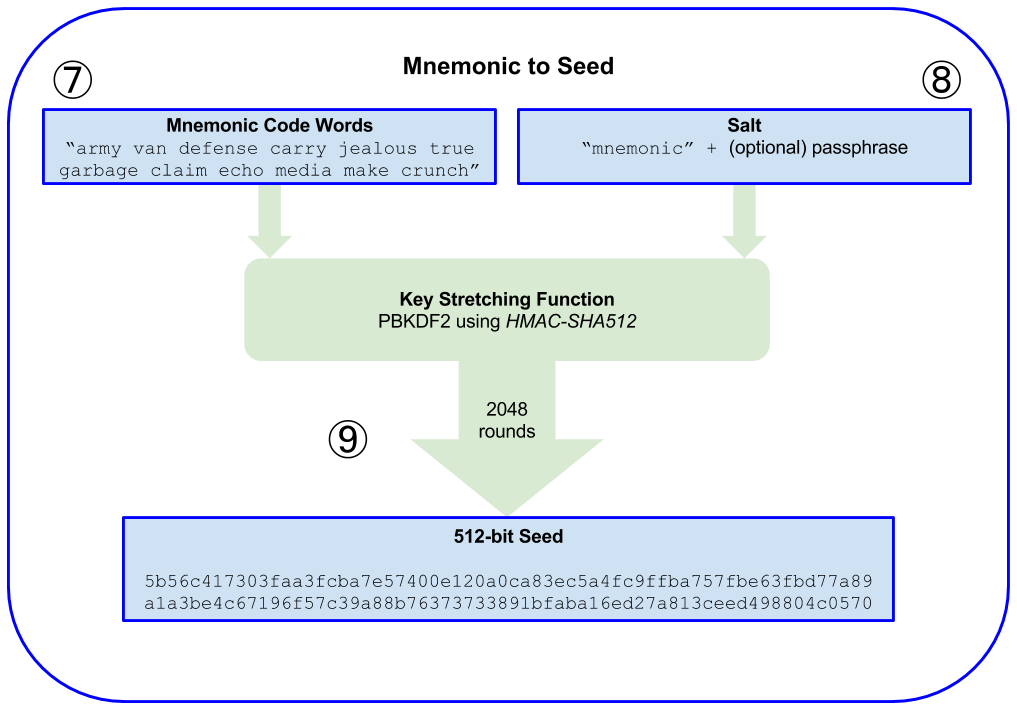
\includegraphics[scale=0.3,clip=false]{pictures/mnemonic-to-seed.png}
  \end{center}

\end{frame}

\begin{frame}\frametitle{Practical considerations}

  \begin{itemize}
  \item keep the mnemonic on paper, never in digital form
  \item memorize the passphrase
  \item let somebody else memorize the passphrase
  \item hint towards a wrong passphrase, leading to a \emph{duress wallet}
  \end{itemize}

\end{frame}

\begin{frame}\frametitle{Parent to child key derivation (BIP-32)}

  \begin{itemize}
  \item there is an algorithm to derive private child keys from private parent keys
  \item there is an algorithm to derive public child keys from public parent keys
    \begin{itemize}
    \item ideal for storing public keys only in a cloud server
    \end{itemize}
  \item the derivation can be \emph{hardened}, so that
    the knowledge of a single private key does not allow to reconstruct
    the other private keys
  \end{itemize}

  \begin{center}
    \begin{tabular}{ll}
      HD path & Key described \\\hline
      \<m/0> & The first (\<0>) child private key of the master private key (\<m>) \\
      \<m/0/0> & The first grandchild private key of the first child (\<m/0>) \\
      \<m/0'/0> & The first normal grandchild of the first \emph{hardened} child (\<m/0'>) \\
      \<m/1/0> & The first grandchild private key of the second child (\<m/1>) \\
      \<M/23/17/0/0> & The first great-great-grandchild public key of the first \\
                     & great-grandchild of the 18th grandchild of the 24th child
    \end{tabular}
  \end{center}
\end{frame}

\begin{frame}\frametitle{Giving structure to the key hierarchy (BIP-44)}

  \begin{center}
    \<[m|M]/purpose'/coin\_type'/account'/change/address\_index>
  \end{center}

  \bigskip

  \begin{greenbox}{}
    The value of \<purpose> is fixed to \<44>.
    For Ethereum, \<coin\_type> is fixed to \<60> and \<change> is fixed to \<0>:
    \begin{center}
      \<[m|M]/44'/60'/account'/0/address\_index>
    \end{center}

    \begin{center}
      \begin{tabular}{ll}
        HD path & Key described \\\hline
        \<M/44'/60'/0'/0/2> & The third public key for the primary\\
                            & Ethereum account\\
        \<M/44'/0'/3'/1/14> & The 15th change-address public key\\
                            & for the 4th Bitcoin account\\
        \<m/44'/2'/0'/0/1>  & The second private key for the primary\\
                            & Litecoin account
      \end{tabular}
    \end{center}
  \end{greenbox}
\end{frame}

\begin{frame}\frametitle{Blocks and transactions}

  \begin{center}
    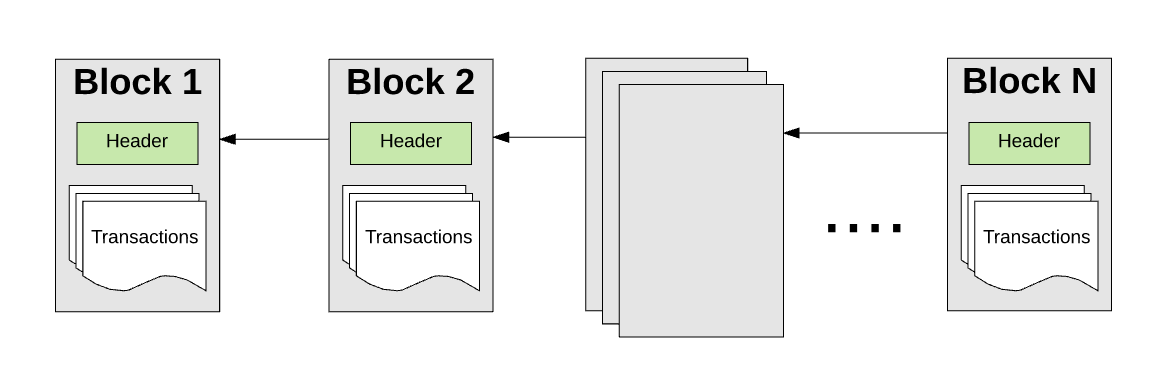
\includegraphics[width=\textwidth,clip=false]{pictures/blocks-contain-transactions.png}
  \end{center}

\end{frame}

\begin{frame}\frametitle{An Ethereum transaction}

  \begin{greenbox}{}
    A transaction is a signed message originated by an EOA, transmitted
    by the Ethereum network, and recorded on the Ethereum blockchain.
    \begin{itemize}
    \item Nonce: sequence number per each originating EOA
    \item Gas price: maximum willing to pay
    \item Gas limit: maximum willing to consume
    \item To: recipient (destination address)
    \item Value: ether sent to destination
    \item Data: generic payload (method name, parameters, contract code\ldots)
    \item v,r,s: ECDSA signature of the originating EOA
    \end{itemize}
  \end{greenbox}

  \begin{center}
    The originating EOA is implied by v,r,s
  \end{center}

\end{frame}

\begin{frame}\frametitle{Transactions induce state transitions}

  \begin{center}
    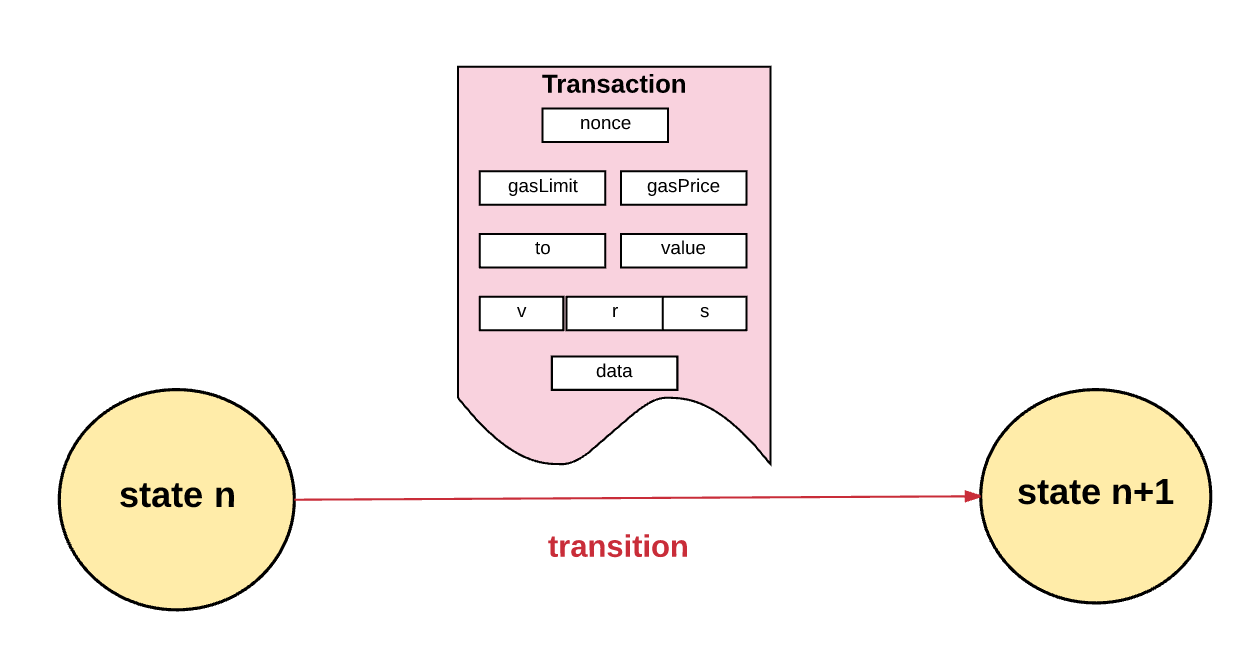
\includegraphics[width=\textwidth,clip=false]{pictures/state-transition.png}
  \end{center}

\end{frame}

\begin{frame}\frametitle{The nonce}

  \begin{greenbox}{The nonce of an EOA}
    A scalar value equal to the number of transactions sent from the EOA.
  \end{greenbox}

  \bigskip

  \begin{greenbox}{Wallets keep track of nonces}
    They increase it and attach to each transaction they create per
    originating EOA.
  \end{greenbox}

  \bigskip

  \begin{greenbox}{Nodes check nonces}
    They count the number $n$ of transactions originated
    by the originating EOA. If the nonce is smaller than $n+1$, the
    transaction is rejected. If the nonce is greater than $n+1$,
    the transaction is delayed and not yet executed:
    \begin{itemize}
    \item this guarantees transaction ordering
    \item and avoids transaction replaying
    \end{itemize}
  \end{greenbox}

  \bigskip

  \begin{redbox}{}
    Keeping track of nonces is hard for concurrent accesses!
  \end{redbox}

\end{frame}

\begin{frame}\frametitle{Computing next nonce in Java using Infura}

  \begin{center}
    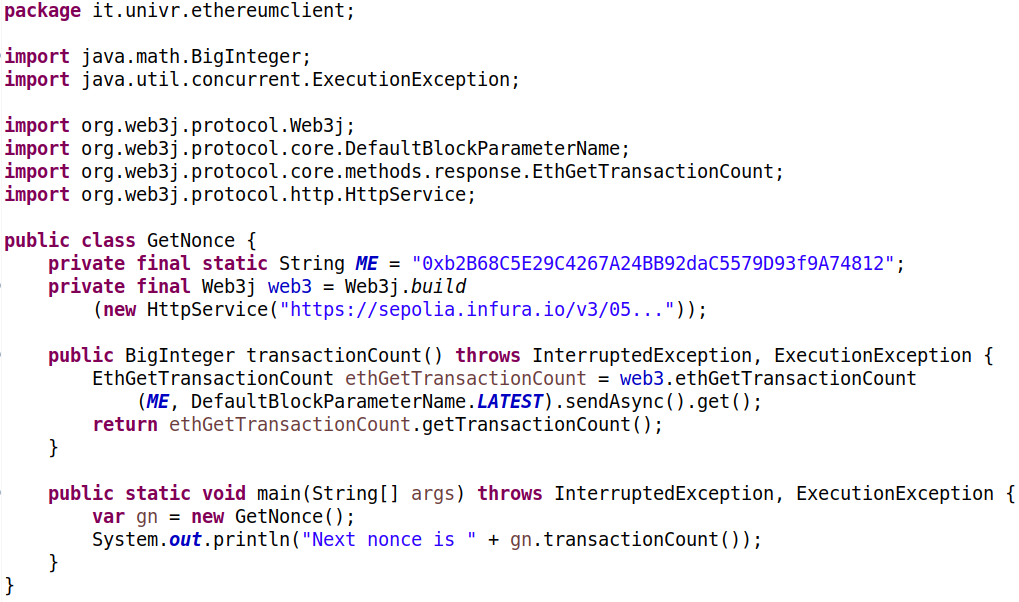
\includegraphics[width=\textwidth,clip=false]{pictures/get-nonce-java.png}
  \end{center}

\end{frame}

\begin{frame}\frametitle{Gas}

  The price of gas fluctuates, for protection against ETH spikes.

  \bigskip

  \begin{greenbox}{\url{https://ethgasstation.info/}}
    \begin{center}
      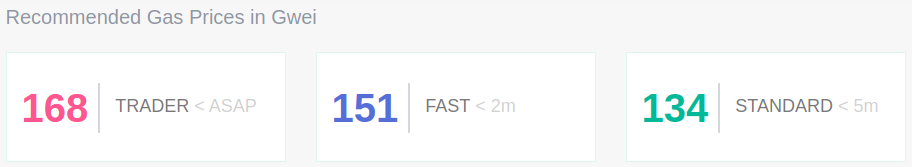
\includegraphics[width=\textwidth,clip=false]{pictures/ethgasstation.png}
    \end{center}
  \end{greenbox}

  \bigskip

  It is well possible that transaction with $0$ gas price will be eventually
  processed.

  \bigskip

  The maximal gas cost of a transaction will be $\mathit{Gas\ price}\times\mathit{Gas\ limit}$.
\end{frame}

\begin{frame}\frametitle{To}

  Any $20$ bytes recipient address can be specified (EOA or contract),
  there is no control!

  \bigskip

  \begin{redbox}{Burning ETH}
    Sending ether to a nonexistent address means \emph{burning} that ether,
    since it's practically impossible to identify the private key
    that controls that address. It is standard practice to burn ether
    by sending it to the address
    \begin{center}
      \<0x000000000000000000000000000000000000dEaD>
    \end{center}
  \end{redbox}

  \bigskip

  Clients should check for correctness of addresses, for instance
  through EIP-55.
\end{frame}

\begin{frame}\frametitle{Signing and sending a transaction in Java with Infura}

  \begin{center}
    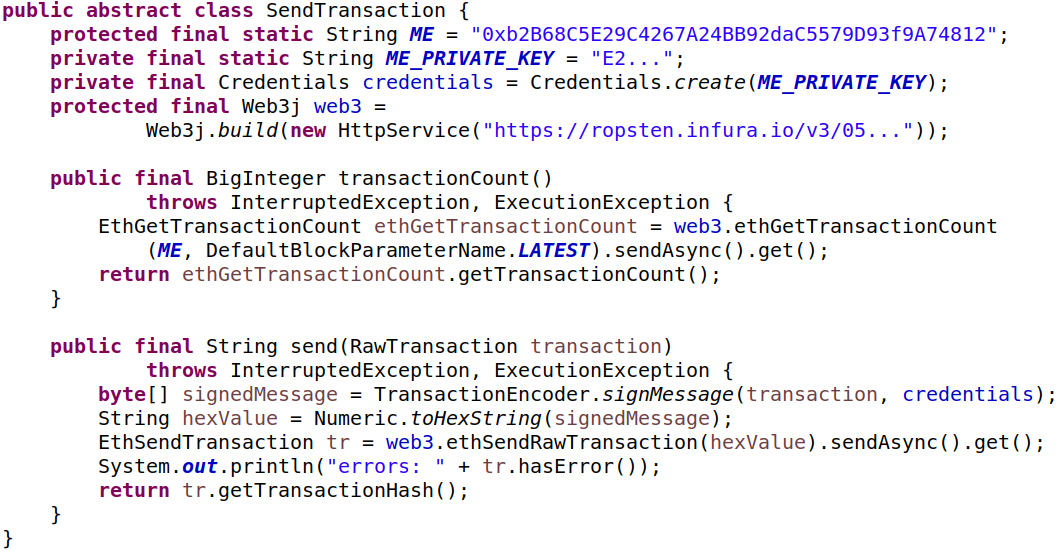
\includegraphics[width=\textwidth,clip=false]{pictures/send-transaction-java.png}
  \end{center}

\end{frame}

\begin{frame}\frametitle{Example: sending ETH from our account to the faucet}

  \begin{center}
    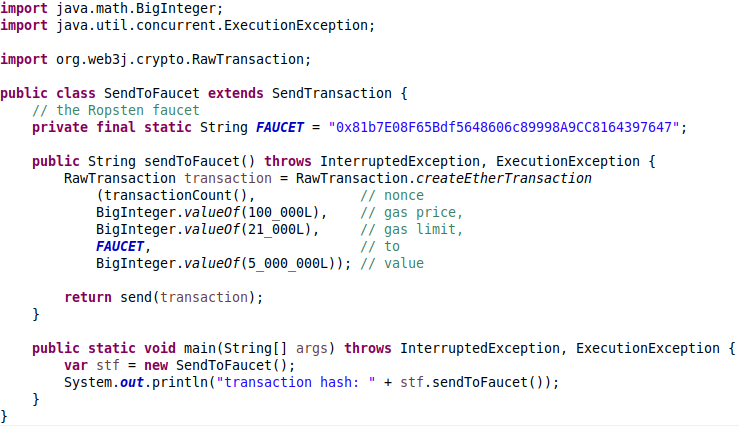
\includegraphics[width=\textwidth,clip=false]{pictures/send-ether-transaction-java.png}
  \end{center}

\end{frame}

\begin{frame}\frametitle{Transactions with value (\emph{payments})}

  \begin{itemize}
  \item the recipient is an EOA (data will be kept in blockchain, but not used)
    \begin{itemize}
    \item the EOA existed already: its balance gets increased by value
    \item the EOA didn't exist before: its balance is set to value
    \end{itemize}
  \item the recipient is a contract
    \begin{itemize}
    \item there is data: the payable method specified by the data will be executed,
      after increasing the contract's balance by value
    \item there is no data
      \begin{itemize}
      \item there is a payable \emph{fallback} function: it will be executed after
        increasing the contract's balance by value
      \item there is no fallback function: the balance of the contract gets increased by value
      \end{itemize}
    \end{itemize}
  \end{itemize}

\end{frame}

\begin{frame}\frametitle{Transactions targetting contract methods}

  \begin{itemize}
  \item the signing key specifies the caller
  \item the recipient specifies the receiver contract of the call
  \item the data component specifies signature and actual arguments of the call
  \end{itemize}

  \bigskip

  \begin{greenbox}{How data is computed}
  \begin{enumerate}
  \item take the callee's signature as a string: \<withdraw(uint256)>
  \item compute its Keccak256 hash
  \item take the first 4 bytes: this is the \emph{function selector}
  \item append the actual arguments, serialized
  \end{enumerate}
  \end{greenbox}

\end{frame}

\begin{frame}\frametitle{Example: call \<withdraw()> on contract installed with Remix}

  \begin{center}
    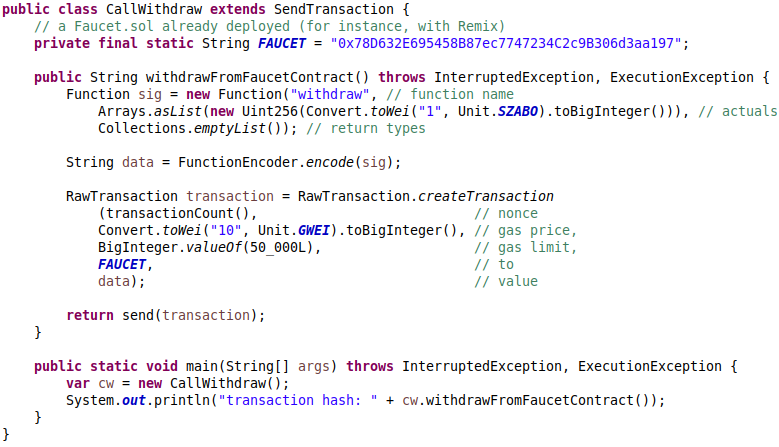
\includegraphics[width=\textwidth,clip=false]{pictures/send-function-transaction-java.png}
  \end{center}

\end{frame}

\begin{frame}\frametitle{Transactions creating a new instance of a contract}

  \begin{itemize}
  \item the signing key specifies the caller
  \item the recipient is set to the zero address
  \item the data component contains the compiled bytecode of the contract
  \item the transaction receipt contains the address of the new contract
  \end{itemize}

  \bigskip

  \begin{redbox}{}
    If the same code is deployed more times, it is \underline{not}
    shared among all instances of the contract. That is, there is no
    notion of classpath in Ethereum.
  \end{redbox}

\end{frame}

\begin{frame}\frametitle{Example: create an instance of \<Faucet.sol> with Infura}

  \begin{center}
    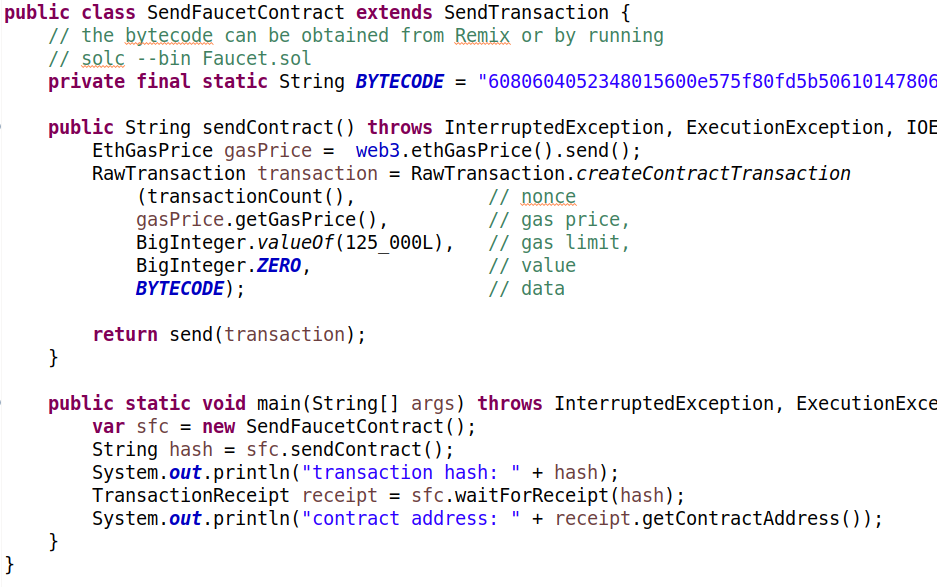
\includegraphics[width=\textwidth,clip=false]{pictures/send-contract-transaction-java.png}
  \end{center}

\end{frame}

\begin{frame}\frametitle{Waiting for the receipt}

  \begin{center}
    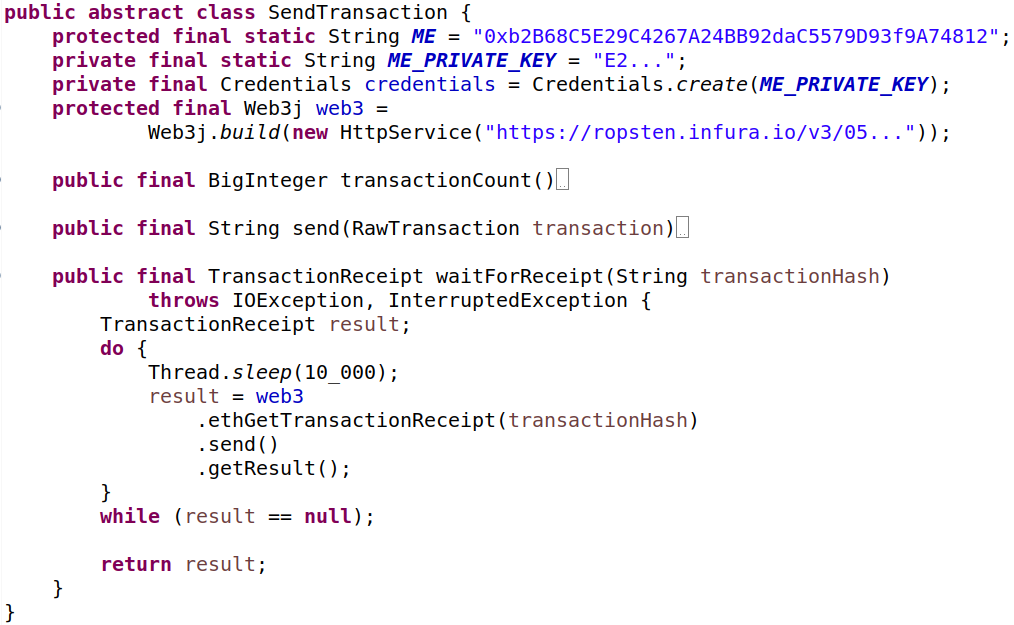
\includegraphics[width=\textwidth,clip=false]{pictures/wait-receipt-java.png}
  \end{center}

\end{frame}

\begin{frame}[fragile]\frametitle{Transaction signing (ECDSA)}

  Transactions are digitally signed before being broadcast to Ethereum:

{\small\begin{verbatim}
Credentials credentials = Credentials.create(ME_PRIVATE_KEY);
byte[] signedMessage = TransactionEncoder.signMessage
  (transaction, credentials);
\end{verbatim}}

  The signature serves three goals:
  \begin{enumerate}
  \item it guarantees that the transaction was created by the sender (\alert{authenticity})
  \item it guarantees that the sender cannot deny having sent the transaction (\alert{non-repudiation})
  \item it guarantees that the transaction was not altered in transit (\alert{integrity})
  \end{enumerate}

  \bigskip

  \begin{greenbox}{}
    The public key of the signer can be recovered from the signed transaction.
    A numerical chain identifier is added to the transaction before signing,
    so that transactions cannot be replayed across networks
    (mainnet, testnets\ldots).
  \end{greenbox}
\end{frame}

\begin{frame}\frametitle{Offline signing}

  \begin{greenbox}{}
    For extreme security, transactions might be signed offline,
    on an \emph{airgapped} computer, so that private keys are not
    in memory of any connected computer.
  \end{greenbox}

  \bigskip

  \begin{center}
    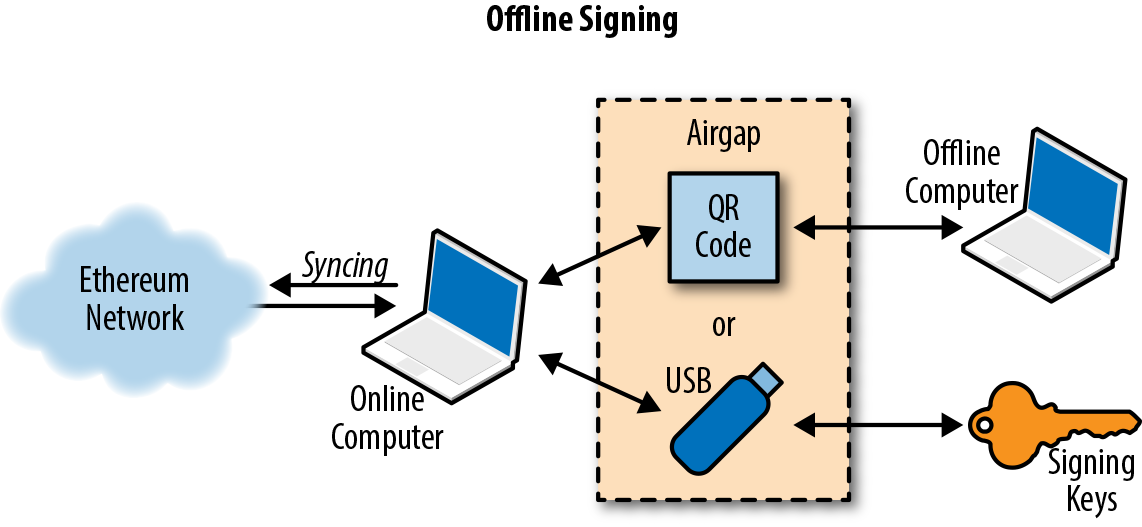
\includegraphics[width=\textwidth,clip=false]{pictures/offline_signing.png}
  \end{center}

\end{frame}

\begin{frame}\frametitle{Transaction broadcasting}

  \begin{greenbox}{}
    Clients broadcast signed transactions to a set of nodes they are in contact with.
    These verify signature and syntax of the transactions and further propagate the signed transactions
    to their neighbors, in a pure P2P approach.
  \end{greenbox}

  \bigskip

  \begin{center}
    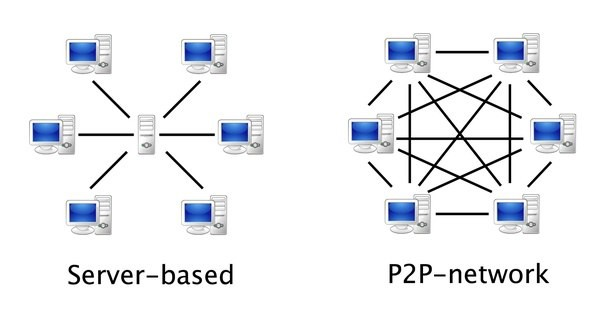
\includegraphics[scale=0.5,clip=false]{pictures/p2p.jpg}
  \end{center}

\end{frame}

\begin{frame}\frametitle{Multi-signature transactions}

  \begin{greenbox}{}
    Differently from Bitcoin, Ethereum has no native support for multi-signature transactions,
    that are only valid if signed by more EOAs. However,
    multi-signature and other signature schemes can be programmed through smart contracts:

    \begin{itemize}
    \item extreme flexibility
    \item risk of bugs
    \end{itemize}
      
  \end{greenbox}

  \bigskip

  \begin{center}
    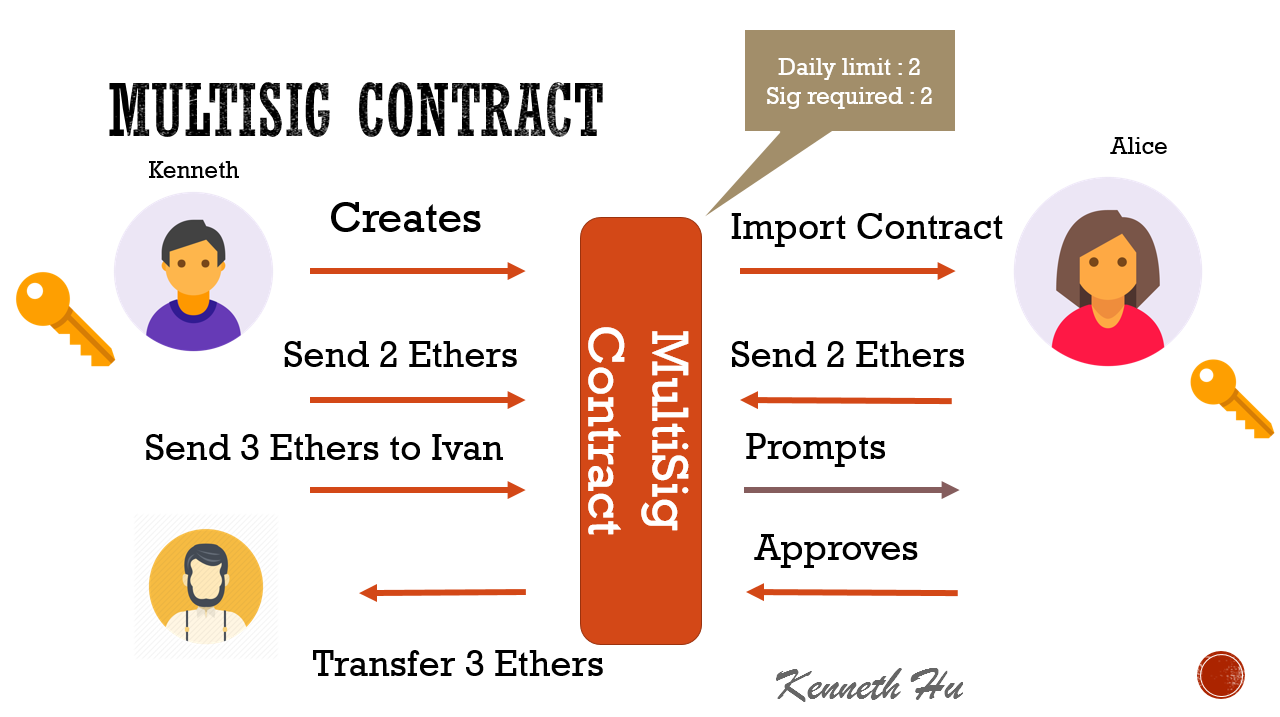
\includegraphics[scale=0.15,clip=false]{pictures/multi-signature.png}
  \end{center}

\end{frame}

\end{document}
